\documentclass{beamer}
\usepackage{ctex} % To support Chinese characters, if needed
\usepackage{graphicx} % To include images
\usepackage{hyperref} % To include hyperlinks
\usepackage{amsmath} % For mathematical symbols
\usepackage{booktabs} % For beautiful tables

% Theme choice:
\usetheme{Madrid}
\usecolortheme{seahorse}

% Custom block colors
\setbeamercolor{block title}{bg=blue!30,fg=black}
\setbeamercolor{block body}{bg=blue!10,fg=black}
% \setbeamercolor{alertblock title}{bg=red!50,fg=white}
% \setbeamercolor{alertblock body}{bg=red!20,fg=black}
\setbeamercolor{exampleblock title}{bg=green!50,fg=black}
\setbeamercolor{exampleblock body}{bg=green!20,fg=black}

% Enable figure numbering
\setbeamertemplate{caption}[numbered]


% Title, author, and date information:
\title{\textbf{Learning Research}}
\author[xjh]{Jiahao Xiang\inst{1}}
\institute{
    \inst{1}
    Hengyang Normal University
}
\date{\today}

\begin{document}

\begin{frame}
    \titlepage
\end{frame}

\begin{frame}
    \frametitle{Preface}
    % introduce the share speech motivation
    \textbf{Motivation:} 对于接触Research一年多,还是小白的我来说,不具备一套高效的方法论。这次分享,我们对常年混迹与顶会的,一位浙大的大佬(彭思达)分享的\texttt{learning\_research}进行学习,在大佬的输入下,输出一下我们学习到的内容,希望能够对大家也有所帮助。
    \vfill
    \begin{block}{大佬思想使用该颜色块标注}
        \url{https://github.com/pengsida/learning_research}
    \end{block}
    \begin{exampleblock}{我们的想法}
        汇报 slide: \url{https://github.com/jiahaoxiang2000/TempWrite/blob/master/slied/learning_research.pdf}
    \end{exampleblock}
    
    
\end{frame}

\begin{frame}
    \frametitle{Table of Contents}
    \tableofcontents
\end{frame}

\section{找问题}
\begin{frame}
    \frametitle{找问题}
    \begin{block}{一阶段}
        这个阶段追求\textcolor{blue}{广度},了解一些基础的概念和算法。不要求深度,不要求掌握/熟悉算法所有的细节。这个阶段的目的是让你对大方向有一个大概的了解,知道有哪些算法,知道这些算法的\textcolor{blue}{大概原理},知道这些算法的应用场景。
    \end{block}
    \begin{block}{二阶段}
        这个阶段追求\textcolor{blue}{深度},追求掌握某一篇论文的细节(算法细节、代码实现细节)。这个阶段的目标是构建某一个科研细分方向的算法基础,了解一篇\textcolor{red}{论文}是怎么做出来的(寻找科研问题、想idea、做实验、写论文)。
    \end{block}
    \begin{exampleblock}{找问题}
        当来到二阶段时,一类问题已经明显了,一类为旧的issue,我们阅读的文献;二类为新的issue,属于开创新的贡献。
    \end{exampleblock}

\end{frame}

\section{解问题}
\begin{frame}
    \frametitle{解问题}
    \begin{block}{三阶段}
        在有了一定算法基础以后,开始在实验室的指导下做一个自己一作的Project。这个阶段的目标是通过\textcolor{red}{实践}来学习一篇论文是怎么做出来的。
    \end{block}
    \begin{exampleblock}{想idea}
        想点子的过程,就是尝试去解问题的过程。找找旧的解法,看看有没有可以改进的地方,或者能不能引入一些新的思路。
    \end{exampleblock}
    \begin{block}{杨植麟认为}
        技术的本质就是对方法做\textcolor{red}{组合},把小的技术组合成大的技术,把老的技术组合成新的技术。
    \end{block}
\end{frame}

\begin{frame}
    \frametitle{想idea}
    具体的想idea的流程(Goal-driven research)
    \begin{block}{1. general goal}
        一般而言,general goal容易定义,但制定roadmap需要对领域有深刻的理解。可以通过构建literature tree来建立起对该领域的认知。
    \end{block}
    \begin{block}{literature tree}
        \begin{itemize}
            \item 收集相同方向的论文。
            \item 通过阅读论文,梳理出当前方向已有的milestone tasks,并标记提出该\textcolor{red}{task}的第一篇论文(1类novelty)。
            \item 将论文根据milestone tasks进行归类。梳理出有代表性的pipelines,并标记提出该\textcolor{red}{pipeline}的第一篇论文(2类novelty)。
            \item 根据pipeline再细分到novel \textcolor{blue}{module},归类论文(3类novelty)。加一些module改进已有pipeline地工作 (4类novelty)
            \item 随着自己对领域的理解,增加新的milestone tasks。
        \end{itemize}
    \end{block}
\end{frame}

\begin{frame}
    \frametitle{想idea}
    \begin{exampleblock}{novelty的分类}
        创新性越高,它所能影响的文章数量就越多。1类milestone task,2类novel pipeline,3类novel module,4类旧module改进已有pipeline地工作。i.e. \textcolor{blue}{创新性很大程度上,影响文章录用的level。}
    \end{exampleblock}
    \begin{block}{2. 选题}
        根据novelty-tree列出的roadmap,选择有研究空间的task,调研这个task有没有重要的technical challenge。\textcolor{red}{选题是对一个research project影响最大的一步,而不是后面的想方法。}
    \end{block}
    \begin{block}{3. why not work reason?}
        从技术层面上分析现在的pipelines在某个task上不work的原因,在pipeline module层面思考可能的原因,然后在pipeline层面或high-level idea层面思考可能的原因。
    \end{block}

\end{frame}

\begin{frame}
    \frametitle{想idea}
    \begin{block}{4. Innovation}
        \begin{itemize}
            \item 通过看论文、思考、做实验、与人讨论等方式,发现当前的pipeline满足不了哪个指标。找到的“问题”。
            \item 1)寻找有没有解决相似“问题”的论文,看看这些论文里有没有分析导致“问题”的技术原因。2)从论文获得的知识。总结这些论文的分析,形成自己的一套思考。3)从有经验的人身上蒸馏知识。4)从实验获得知识。
        \end{itemize}
    \end{block}
    \begin{exampleblock}{找点子}
        点子函数$f:g\mapsto q$, 其中$g$为具有泛化性的知识,i.e. 可以用在多个问题上,$q$为具体的问题。我们的目标是找到一个函数$f$,使得$q$尽可能优。

        1)知$f_1:g\mapsto q_1,q_1\approx q_2$,求$f_2:g\mapsto q_2$。2)和3)知$q$,找$g$,求$f$。4)知$q,g$,求$f$。\textcolor{blue}{2)和3)难,1)简单一些}。
    \end{exampleblock}
    5. 实验验证创新点。
\end{frame}

\begin{frame}
    \frametitle{想idea}
    \begin{block}{Goal-driven research在research产出方面的好处}
        Goal-driven research的风格是追求重要的任务,试各种方法把这个任务做work。通过一些条件的relax,总可以把一些重要的任务做出一些work的结果。这样project有\textcolor{red}{产出的保证}。

        有些人喜欢追新技术,一味的把新技术调work。但我们这方向是实验科学,不通过大量实验难以确定一个技术是否真的work,导致这种科研方式风险性太大了。
    \end{block}
    \begin{block}{当出现新锤子的时候}
        非常值得拿新锤子来做自己roadmap上的某一个milestone task,这样容易做出有影响力的工作。如:
        \begin{itemize}
            \item Transformer出来的时候,拿来搞LoFTR
            \item NeRF出来的时候,拿来搞Neural Body
            \item Stable diffusion出来的时候,拿来搞DreamFusion、DreamBooth
        \end{itemize}
    \end{block}
\end{frame}

\begin{frame}
    \frametitle{想idea}
    \begin{block}{实验室的帮助}
        \begin{itemize}
            \item 开箱自带重要的科研问题 task。
            \item 丰富的Review经验。
            \item 防止进入local minimum,路走窄。
            \item 避免technical flaw,路走死。
            \item 帮改进其提出的创新。
        \end{itemize}
    \end{block}
\end{frame}


\section{做实验}

\begin{frame}
    \frametitle{做实验}
    \begin{figure}[h]
        \centering
        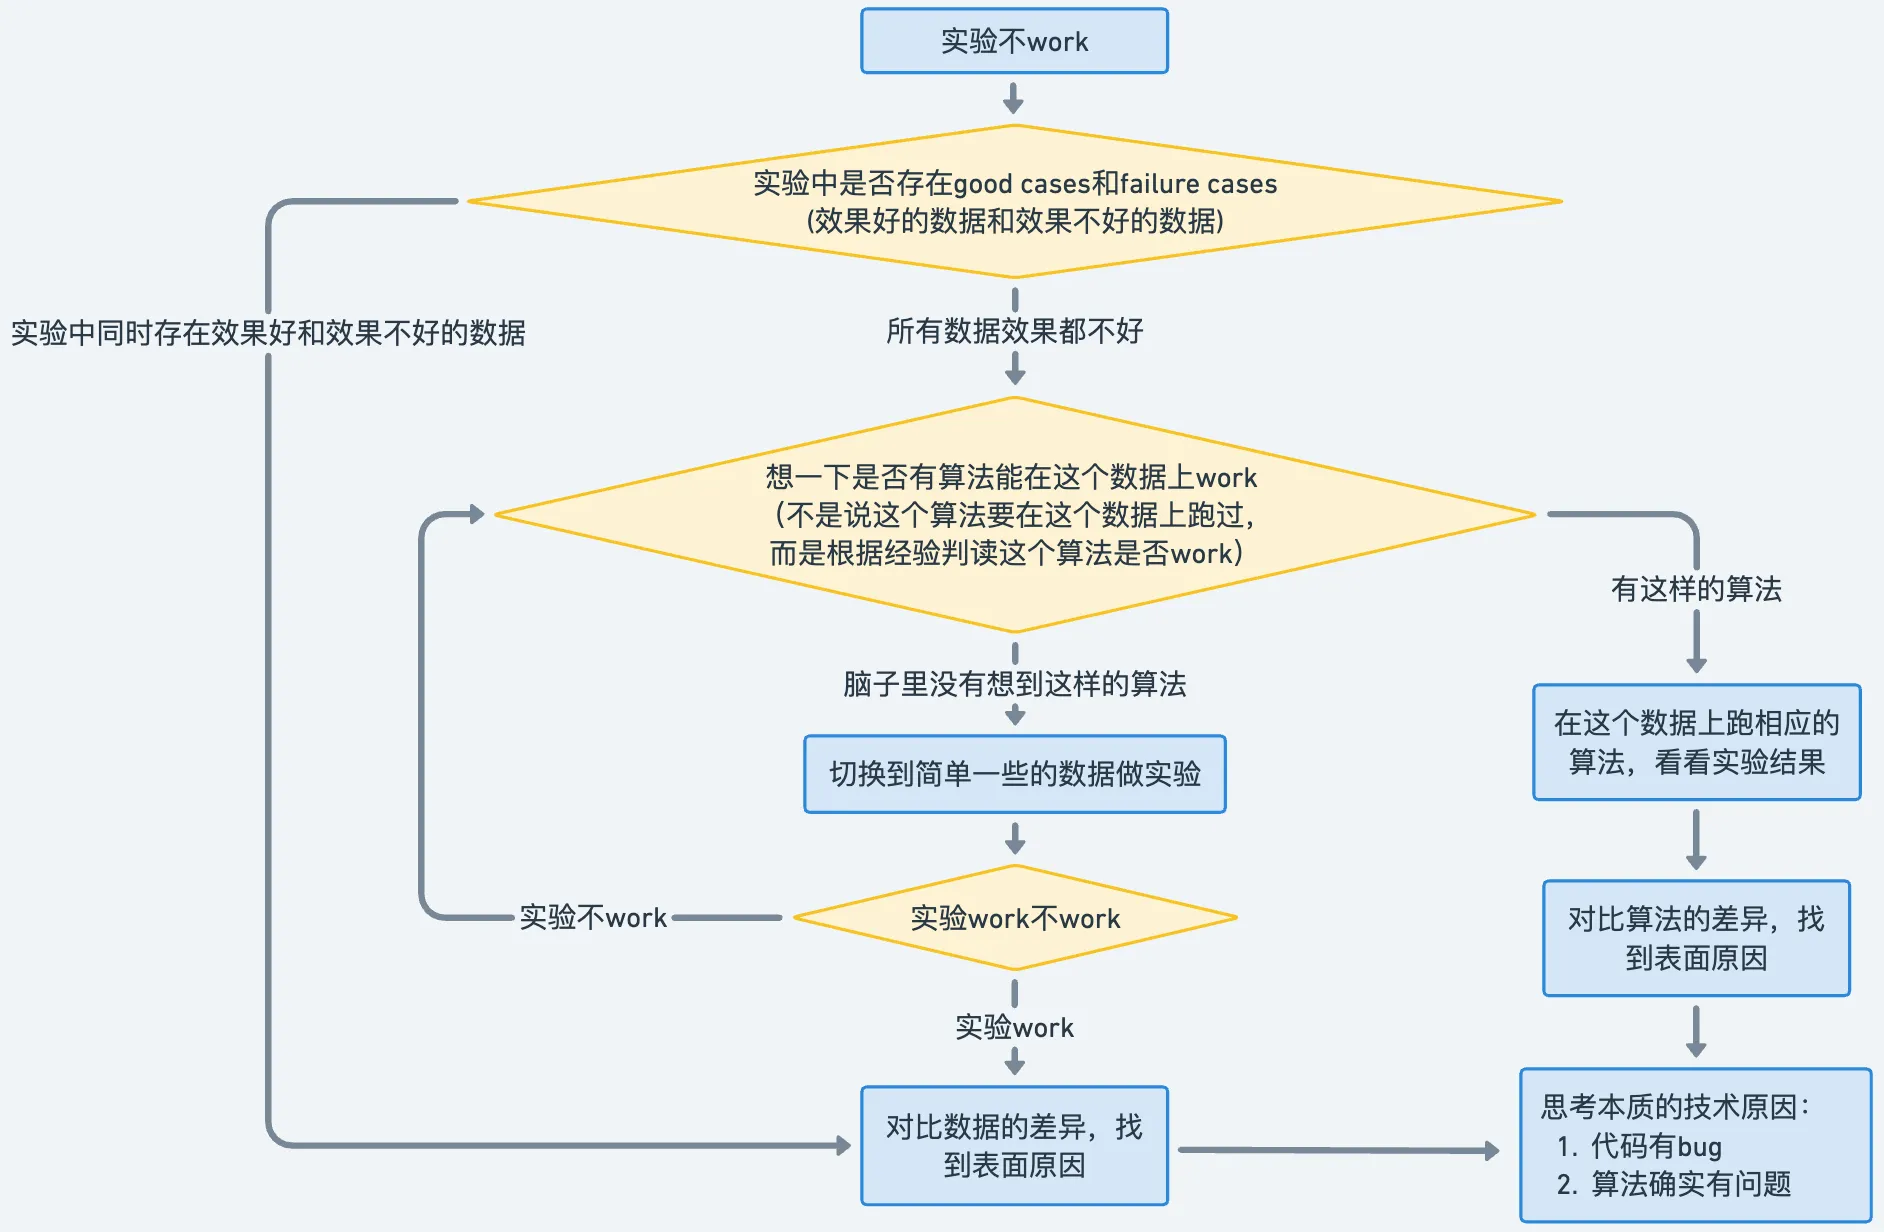
\includegraphics[width=0.8\textwidth]{figure/idea_not_work.png}
        \caption{如何找到当前实验不work的原因}
        \label{fig:experiment}
    \end{figure}
\end{frame}


\begin{frame}
    \frametitle{做实验}
    \begin{block}{not work怎么办}
        \begin{enumerate}
            \item 搜集当前实验的failure cases
            \item 搜集当前实验的good cases(效果好的实验结果),或者找到一个能work的实验版本。方式:\textcolor{blue}{降低问题复杂度,遍历问题点。}
            \item 分析“work的实验版本”和“不work的实验版本”之间存在performance gap的技术原因。\textcolor{red}{列出尽量多的技术原因。}
            \item 实验验证上一步中提出的技术原因。\textcolor{red}{快速迭代。}
            \item 针对导致failure cases的技术原因,提出解法。(需要建立自己的武器库,知道学术界都有哪些技术。可以通过构建\textcolor{blue}{literature tree}来帮助建立武器库。)
            要经常性地确认自己在正确的方向上:当前的算法思路真的对吗。要避免陷入local minima。建议经常找同学\textcolor{blue}{交流讨论}。
        \end{enumerate}
    \end{block}
\end{frame}

\section{写论文}

\section{搓PPT}

\section{Conclusion}


\end{document}